% +---------------------------------------------------------------------------+
% | CGAL User Manual:  visibility_complex.tex
% +---------------------------------------------------------------------------+
% | Visibility complex. Implemented by topological sweep using the 
% | Greedy Flip Algorithm
% +---------------------------------------------------------------------------+
%% \RCSdef{\vcomplexRev}{$Id$}
%% \RCSdefDate{\vcomplexDate}{$Date$}

\ccParDims

\ccUserChapter{2D Visibility Complex}
\label{chapterVisibilityComplex2}
%% \ccChapterRelease{\vcomplexRev. \ \vcomplexDate}
\ccChapterAuthor{Pierre Angelier \and{} Michel Pocchiola \and{} Luc Habert}

\minitoc

% +----------------------------------------------------------------------------+
\section{Introduction}
\label{sectionVComplexIntroduction}
This package implements the visibility complex structure introduced by
Pocchiola and Vegter in~\cite{pv-vc-96} (see also~\cite{pv-tsvcpt-96}
and~\cite{ap-sstvc-01} for a more recent presentation). Although a
generalization to three dimensional environments has been proposed
in~\cite{ddp-fahrgv-99} we deal here only with planar scenes.

The visibility complex is a 2D cell complex whose 1-skeleton is isomorphic to
the visibility graph.  The visibility graph can be used to compute the shortest
path between two points in a planar scene. A survey on visibility graphs and
shortest paths can be found in~\cite{m-gspno-00}.

Our implementation of the visibility complex structure follows closely the
design of the Halfedge Data Structure (see the introduction in
Chapter~\ref{chapterHalfedgeDS} and~\cite{k-ugpdd-99}) however this chapter
can be understood without reading the corresponding chapter.

We use the so-called Greedy Flip Algorithm (again see~\cite{pv-tsvcpt-96})
to compute the visibility complex in optimal time complexity $O(k + n\log
n)$ where $n$ is the size of the input and $k$ the size of the output
(i.e. the visibility complex).
% +----------------------------------------------------------------------------+
\section{Definitions}
In this section we review the basic concepts defined in~\cite{ap-sstvc-01}
which are useful to understand the basic functionality of the package.

\paragraph{Basic definitions.}
A \emph{disk} is a bounded closed convex subset of the plane and a
\emph{scene} is a collection of pairwise disjoint disks. For the ease of
the exposition we will assume that the disks have non-empty interior and
that the tangent line at a point on the boundary of a disk is well
defined. We will also suppose that our disks are in general position that
is, that there is no line tangent to three disks. Although these
definitions rule out points, segment and polygons our implementation can
handle these types of disks through a symbolic perturbation scheme which is
invisible to the user.  The general position assumption is also lifted
through perturbation.  More details are given in the degeneracies section
below. Note also that non convex polygons are also supported via the use of
\emph{constraints} which are defined further on.

A \emph{bitangent} is a directed line segment tangent to two disks and
intersecting these disks only at its endpoints.  The disk containing the
source and target point of the bitangent are called respectively the source
and target disk.  Two disks share four bitangents directed from the first
towards the second.

\begin{ccTexOnly}
    %\vspace{-7mm}
    \begin{center}
      \parbox{0.4\textwidth}{%
          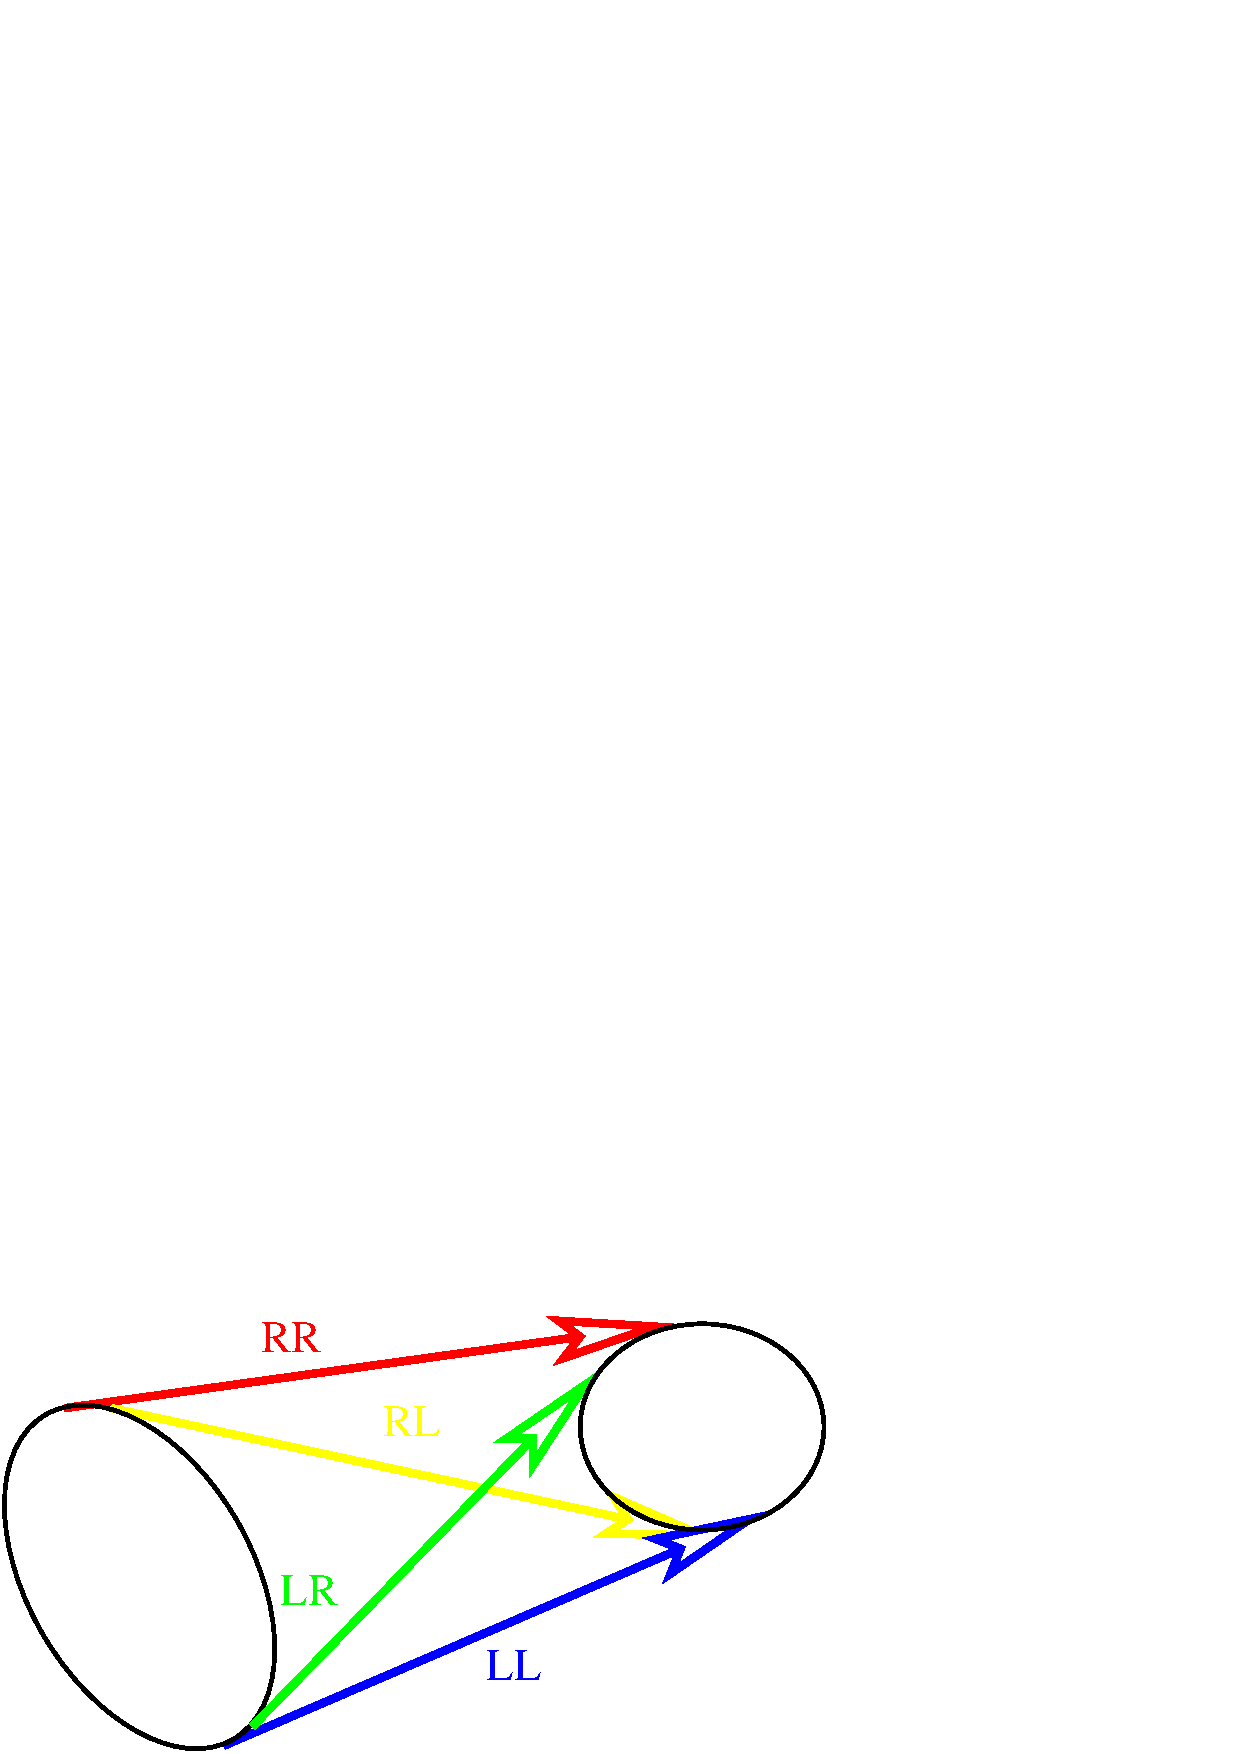
\includegraphics[width=0.4\textwidth]{Visibility_complex_2/fig/bitangent}%
      }
    \end{center}
    %\vspace{-5mm}
\end{ccTexOnly}

\begin{ccHtmlOnly}
    <CENTER>
        <img src="fig/bitangent.gif" alt="Bitangent"><P>
    </CENTER>
\end{ccHtmlOnly}

\label{VC2-bit-type}
The \emph{type} of a bitangent $t$ directed from a disk $A$ to a disk $B$
codes the positions of $A$ and $B$ with respect to the supporting line of
$t$. As illustrated in the Figure above there are four possible types
called \texttt{LL, RR, LR} and \texttt{RL}. A \texttt{LR} bitangent $t$ for
example, is such that $A$ and $B$ lie respectively on the left and on the
right of the supporting line of $t$.

Consider a scene $S$. A bitangent between two disks of $S$ is \emph{free}
if its interior does not intersect a disk of $S$.  A \emph{constrained
scene} $S_H$ is a scene $S$ and a subset $H$ of pairwise non crossing free
bitangents. The bitangents of $H$ are called \emph{constraints}. A
bitangent is \emph{free} in $S_H$ if it is free in $S$ and does not
intersect a bitangent of $H$.  Constraints are still called free bitangents
of $S_H$.

The set of free bitangents tangent to a given disk partition its boundary
into what we call \emph{arcs}. In other words an arc is a portion of the
boundary of a disk defined by two consecutively tangent bitangents.

A \emph{positive arc} belonging to a disk $d$ is an arc whose tangent lines
leave $d$ on its left. The definition of a \emph{negative arc} is obtained
by replacing the word "left" with "right". Thus for each arc we consider
two copies of it: a positive and a negative one. A \emph{signed arc} is a
positive or a negative arc.

\paragraph{Tangent visibility graphs}
Given a constraint scene $S_H$, the \emph{tangent visibility graph} of
$S_H$ is the directed graph where there is:
\begin{itemize}
    \item one vertex per free bitangent of $S_H$.
    \item one edge per signed arc. The edge connects the two vertices
    corresponding to the bitangents defining the arc. A counter-clockwise
    orientation of the boundary of the disks induce an orientation of the
    edges of the visibility graph.
\end{itemize}
Let $e$ be an edge. The two vertices connected by $e$ are denoted $\inf(e)$ and
$\sup(e)$ and are called the source and sink of $e$. These vertices are such
that $e$ is directed from $\inf(e)$ towards $\sup(e)$.

Each vertex of the tangent visibility graph is incident to four edges (two
on the source disk and two on the target disk). The names of these edges
are given in the Figure below.
\begin{ccTexOnly}
    \begin{center}
        \psfrag{v}{$v$}
        \psfrag{ccw_target_edge(v)}{\texttt{ccw\_target\_edge}($v$)}
        \psfrag{cw_target_edge(v)}{\texttt{cw\_target\_edge}($v$)}
        \psfrag{ccw_source_edge(v)}{\texttt{ccw\_source\_edge}($v$)}
        \psfrag{cw_source_edge(v)}{\texttt{cw\_source\_edge}($v$)}
        \psfrag{e}{$e$}
        \psfrag{sup(e)}{$\sup(e)$}
        \psfrag{inf(e)}{$\inf(e)$}
        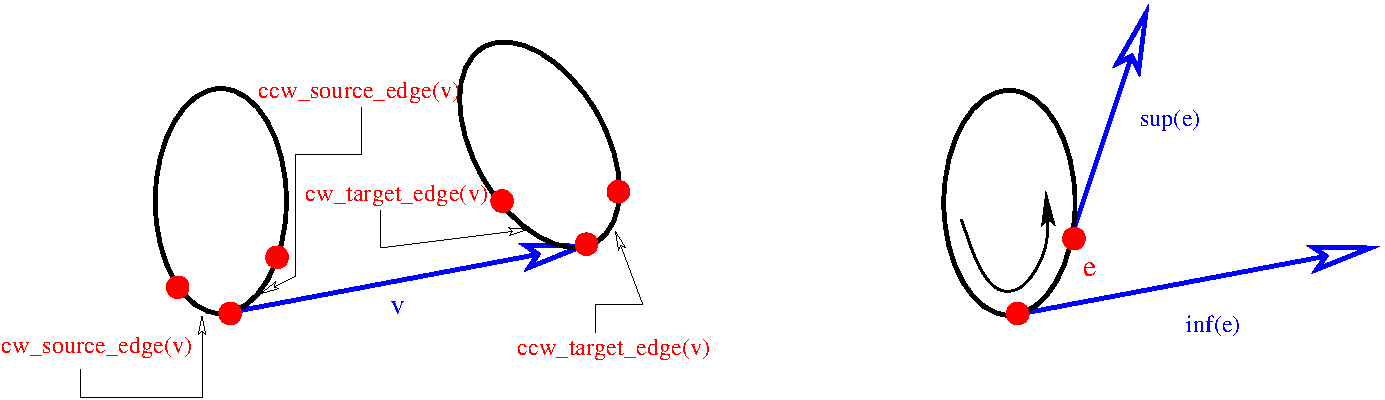
\includegraphics[height=8cm,width=\linewidth]{Visibility_complex_2/fig/edge-vertex}%
    \end{center}
\end{ccTexOnly}

\begin{ccHtmlOnly}
    <CENTER>
        <img src="fig/edge-vertex.gif" alt="Edge-Vertex adjacencies"><P>
    </CENTER>
\end{ccHtmlOnly}

\paragraph{Visibility complexes. }\label{VC2-vcdef}
For more sophisticated visibility queries, the visibility complex is more
appropriate than the tangent visibility graph. It has a richer
two-dimensional cell structure whose 1-skeleton (i.e. the graph obtained by
keeping only the vertex/edges incidences) is exactly the visibility
graph. The definition of the visibility complex is more tricky and requires
the reader to be familiar with the concepts of \emph{equivalence classes},
\emph{quotient space} and the \emph{cutting} of a surface along a
curve. The rest of the definitions of this section can be skipped if one
plans to use only the functionality of the visibility graph (shortest paths
for example).

Consider a constrained scene $S_H$. The \emph{free space} of $S_H$ is the
space obtained by cutting the complement of the interior of the disks of $S$
along the constraints of $H$.

A \emph{ray} is a pair $(p,\alpha)$ consisting of a point $p$ in free space
and a direction $\alpha \in \mathbb{S}^1$ (the 1-sphere).  The
\emph{visibility complex} of a constrained scene $S_H$ is the quotient
space of the set of rays with respect to the following equivalence relation
$\sim$:
\begin{equation}
(p,\alpha) \sim (q,\beta) \textrm{ iff. } \alpha = \beta \textrm{ is the
direction of the line $(p,q)$ and the segment } [p,q] \textrm{ lies in the
free space of } S_H.
\end{equation}
The origins of the rays belonging to a same equivalence class define a
maximal length segment in free space or \emph{maximal segment} for short.
The visibility complex is a two dimensional cell complex. We describe its
elements in the case where the set of constraints is empty. The adjunction
of constraints is discussed later on. The 0,1 and 2-dimensional cells of
the visibility complex are respectively:
\begin{itemize}
    \item \emph{Vertices}: a vertex corresponds to a maximal segment tangent to
    two disks. Each vertex has its associated geometric bitangent.
    \item \emph{Edges}: an edge corresponds to maximal segments tangent to
    one disk and touching the same pair of disks at their extremities. \\
    Let $e$ be an edge corresponding to maximal segments tangent to a disk
    $o$.  If $o$ lies on the left of the supporting line of these segments
    then $e$ is said to be \emph{positive}. Otherwise $e$ is
    \emph{negative}.
    \item \emph{Faces}: a face is the set of maximal segments that touch the
    same pair of disks. The disk containing the source (resp. the target) of 
    these maximal segments is called the backward view (resp. forward view) of 
    the face.
\end{itemize}

\begin{ccTexOnly}
    \begin{center}
        \psfrag{Vertices}{Vertices}
        \psfrag{Edge}{Edge}
        \psfrag{Face}{Face}
        \psfrag{forward view}{forward view}
        \psfrag{backward view}{backward view}
        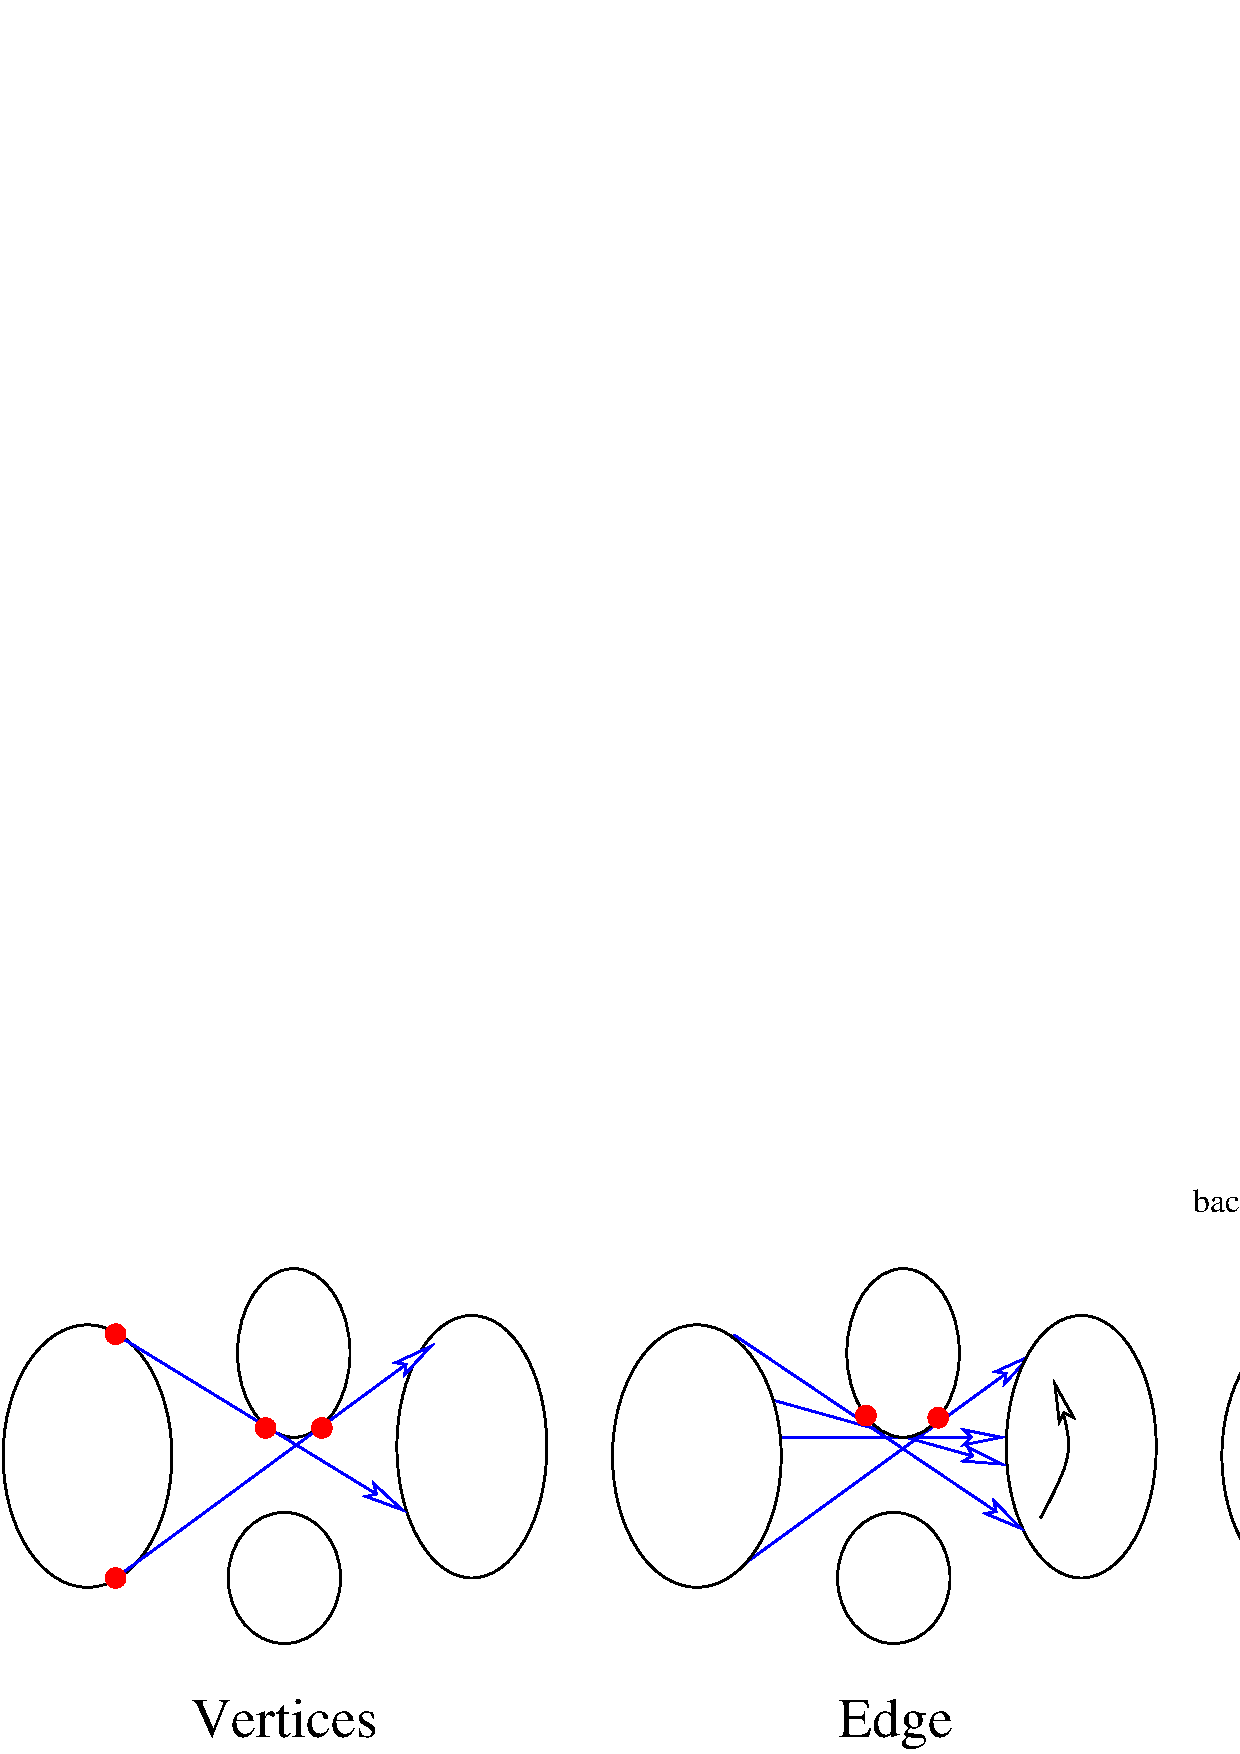
\includegraphics[height=5cm,width=\linewidth]{Visibility_complex_2/fig/vis-complex}%
    \end{center}
\end{ccTexOnly}

\begin{ccHtmlOnly}
    <CENTER>
        <img src="fig/vis-complex.gif" width="90%" 
         alt="The cells of the Visibility Complex"><P>
    </CENTER>
\end{ccHtmlOnly}

The 1-skeleton of the visibility complex is isomorphic to the visibility graph.
The additional information brought by the visibility complex resides in the
faces. Each maximal segment defines an unique face.

We now describe the different incidences between vertices, edges and faces in
the visibility complex. The discussion below is valid for scene that do not
contain constraints. The adjunction of these involves a small change concerning
edges which is discussed later on.
\begin{description}
    \item[{Face--Vertex incidences}]  The number of vertices adjacent
    to a given face $\sigma$ is at least $2$ and at most linear. We offer
    an access to two vertices of particular interest denoted by
    $\sup(\sigma)$ and $\inf(\sigma)$ which are intuitively the segments in
    the face with maximal and minimal angle. More precisely the set of
    maximal segments of a face is ordered by the following relation:
    \begin{equation}
                    a < b \textrm{ iff. } \det(a,b) > 0.
    \end{equation}
    The vertices $\inf(\sigma)$ and $\sup(\sigma)$ are respectively the minimum
    and maximum for this order. 
    %\todo{Warning: convex-hull vertices...}\\
    Each vertex $v$ is incident to six faces. 
    \item[{Edge--Face incidences}]  An edge $e$ is adjacent to three
    faces. These are obtained by taking a maximal segment of the edge and
    moving it slightly. See the figure below for the names of these faces.

    \begin{ccTexOnly}
        \begin{center}
            \psfrag{dl(e)}{dl($e$)}
            \psfrag{dr(e)}{dr($e$)}
            \psfrag{ul(e)}{ul($e$)}
            \psfrag{ur(e)}{ur($e$)}
            \psfrag{e}{$e$}
            \psfrag{Positive edge}{Positive edge}
            \psfrag{Negative edge}{Negative edge}
            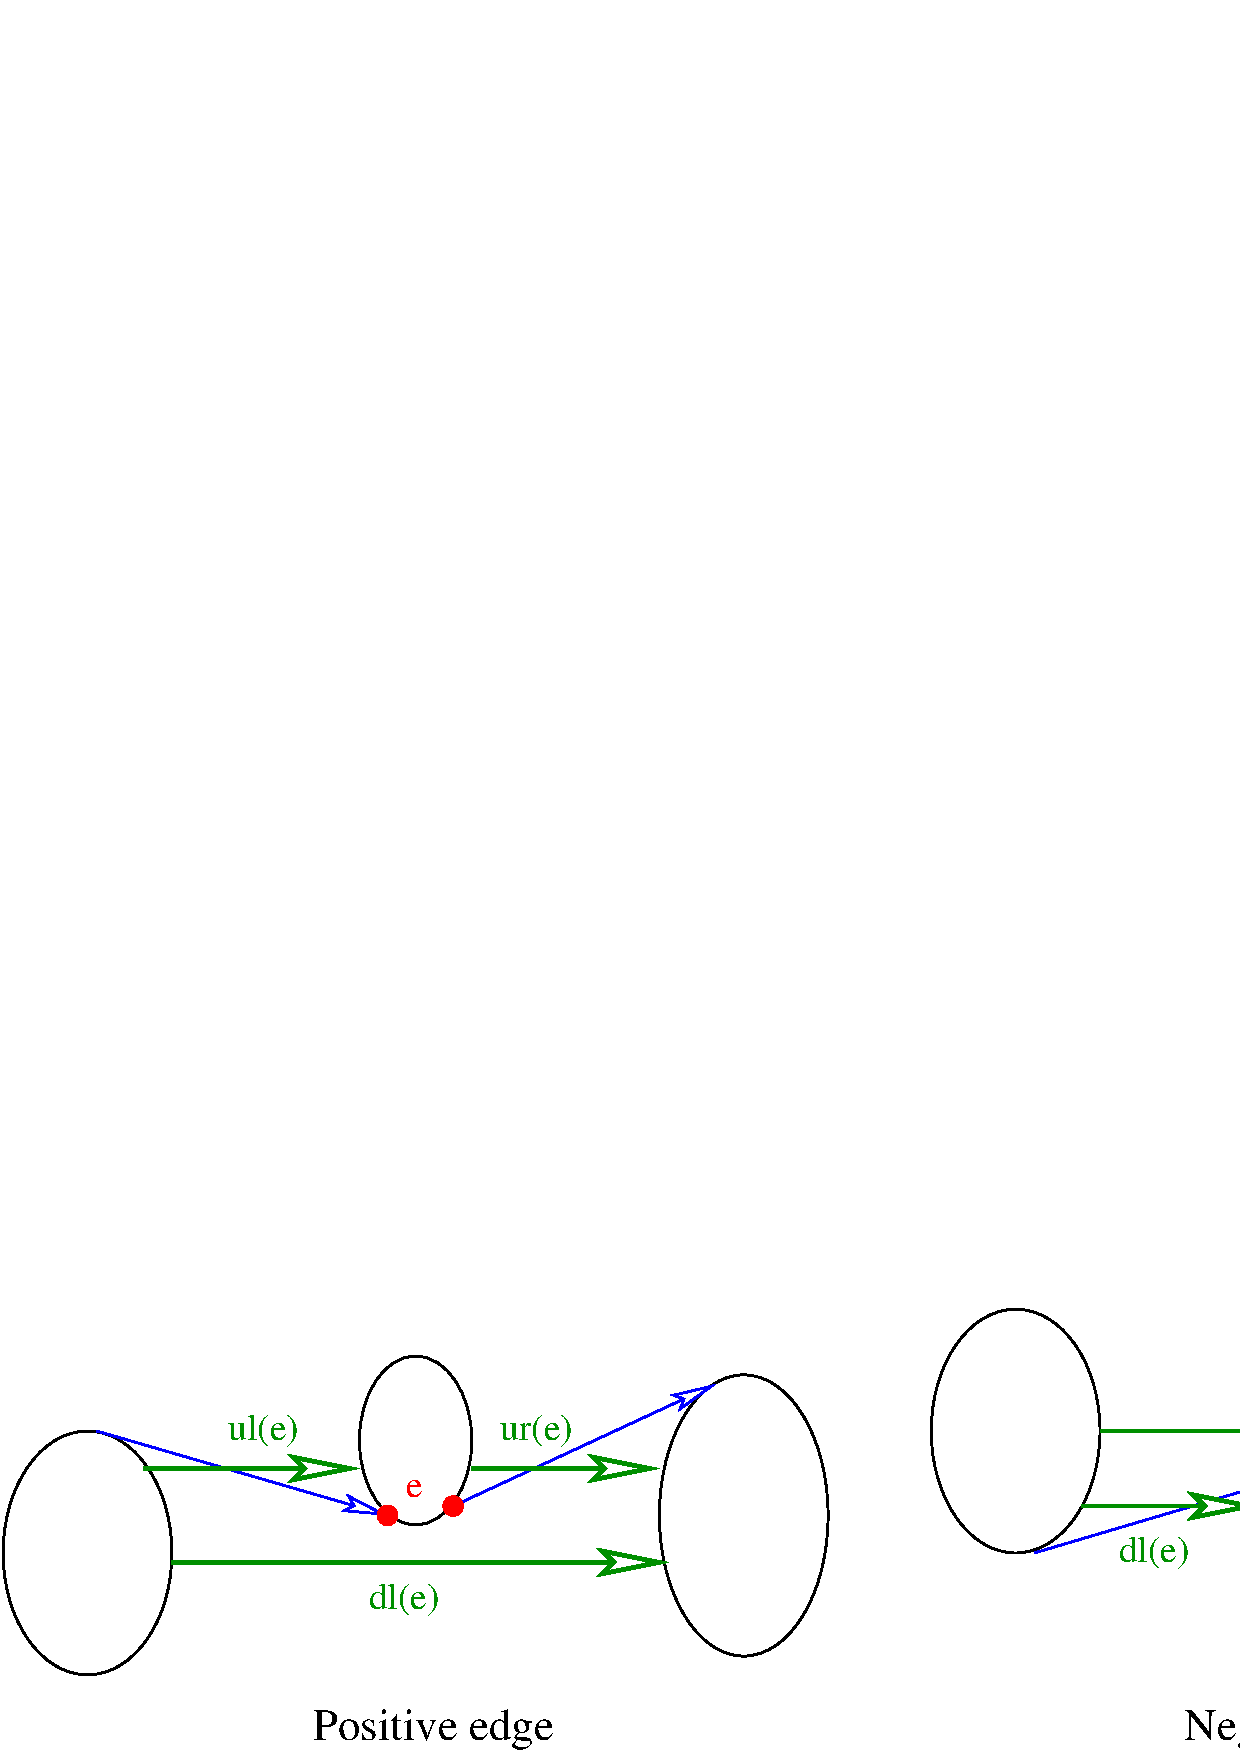
\includegraphics[height=5cm,width=\linewidth]{Visibility_complex_2/fig/edge-face}%
        \end{center}
    \end{ccTexOnly}

    \begin{ccHtmlOnly}
        <CENTER>
            <img src="fig/edge-face.gif" width="90%"
             alt="Edge-Face adjacencies"><P>
        </CENTER>
    \end{ccHtmlOnly}
    For a positive edge $e$ we set dr$(e) = $dl$(e)$ and for a negative edge
    ur$(e) = $ul$(e)$.
    \item[{Edge--Vertex incidences}]These incidences were described in
    the Visibility Graph section above.
\end{description}

We now describe the two main differences brought by the adjunction of
constraints (a more detailed and complete discussion can be found
in~\cite{ap-sstvc-01}).  First, the vertices corresponding to constraints are
adjacent to $8$ faces rather than $6$ before. The other difference is that the
visibility complex also contains special types of edges arousing from rays
emanating from the extremity of a constraint. Such an edge $e$ is called a
\emph{constraint edge} and is adjacent to only one face denoted by face$(e)$.
See the Figure below for an illustration.
\begin{ccTexOnly}
    \begin{center}
        \psfrag{face(e)}{face($e$)}
        \psfrag{e}{$e$}
        \psfrag{constraint}{constraint}
        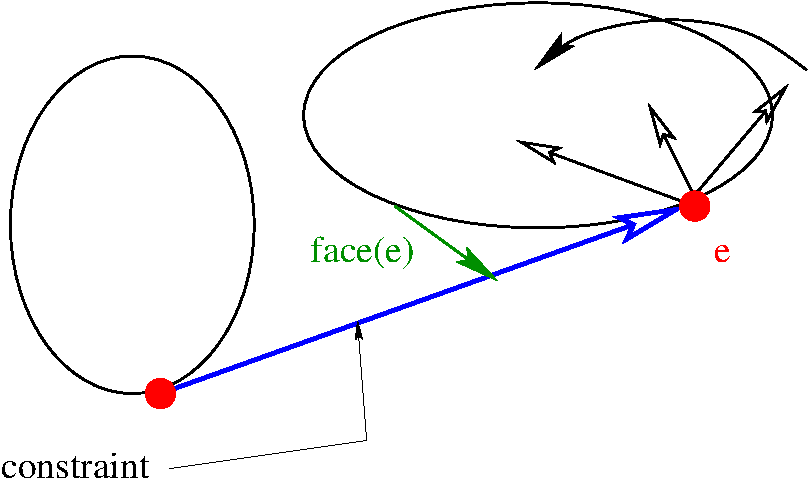
\includegraphics[height=5cm]{Visibility_complex_2/fig/constraint-edge}%
    \end{center}
\end{ccTexOnly}

\begin{ccHtmlOnly}
    <CENTER>
        <img src="fig/constraint-edge.gif" alt="Constraint Edges"><P>
    </CENTER>
\end{ccHtmlOnly}

\paragraph{Degenerate cases.} The above discussion holds for disks which have
non empty interior and a smooth boundary. However, our implementation can
handle points, segments and convex polygons which are what we call
degenerate cases.  This is achieved via a symbolic perturbation obtained by
taking the Minkowski sum of a degenerate disk with a small circle having an
infinitesimal radius.

\begin{ccTexOnly}
    \begin{center}
        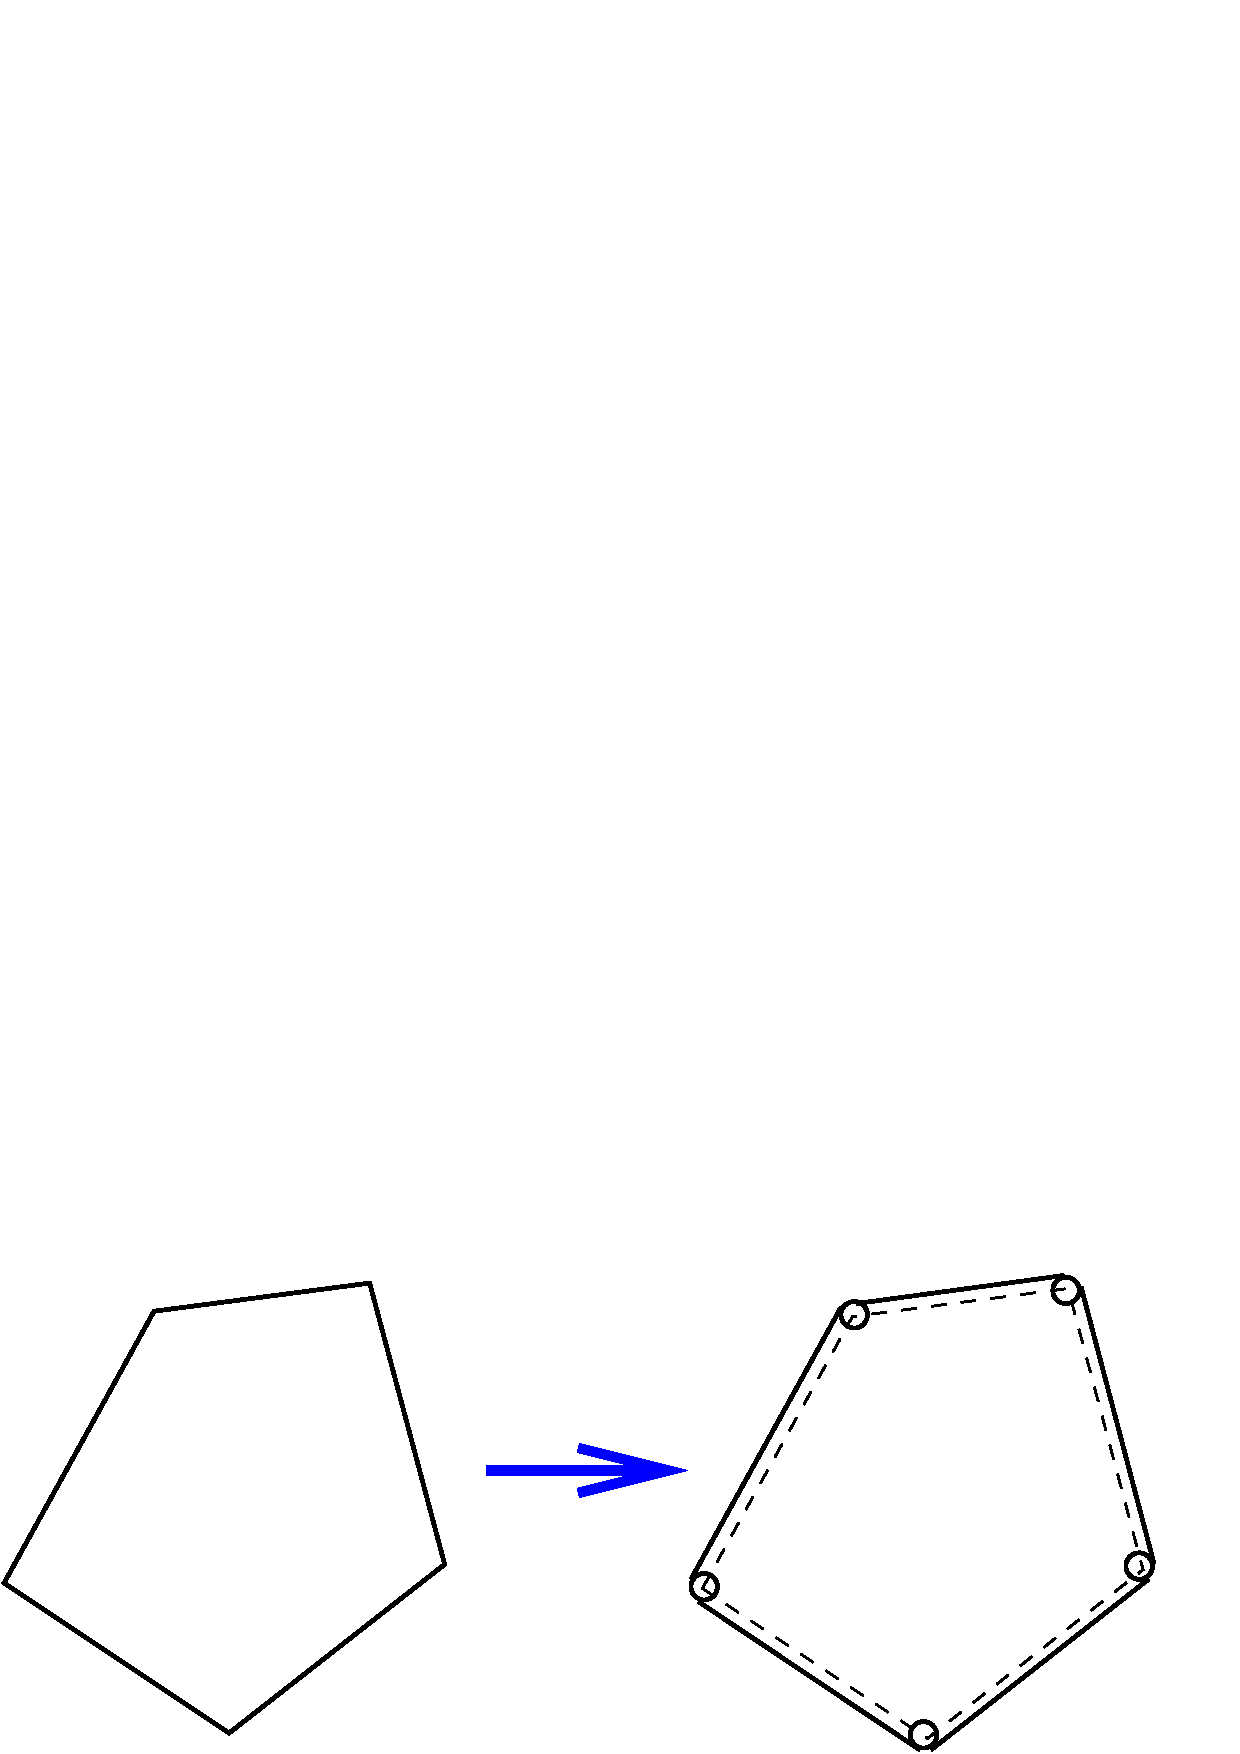
\includegraphics[height=4cm]{Visibility_complex_2/fig/perturbation}%
    \end{center}
\end{ccTexOnly}

\begin{ccHtmlOnly}
    <CENTER>
        <img src="fig/perturbation.gif" alt="Perturbation"><P>
    </CENTER>
\end{ccHtmlOnly}

This perturbation implies no numerical computations and is completely
invisible to the user. Each time a scene contains a degenerate disk, the user
is invited to mentally replace it by its perturbated version in order to
visualize the visibility complex or graph. 

\begin{ccTexOnly}
    \begin{center}
        \psfrag{Perturbation}{Perturbation}
        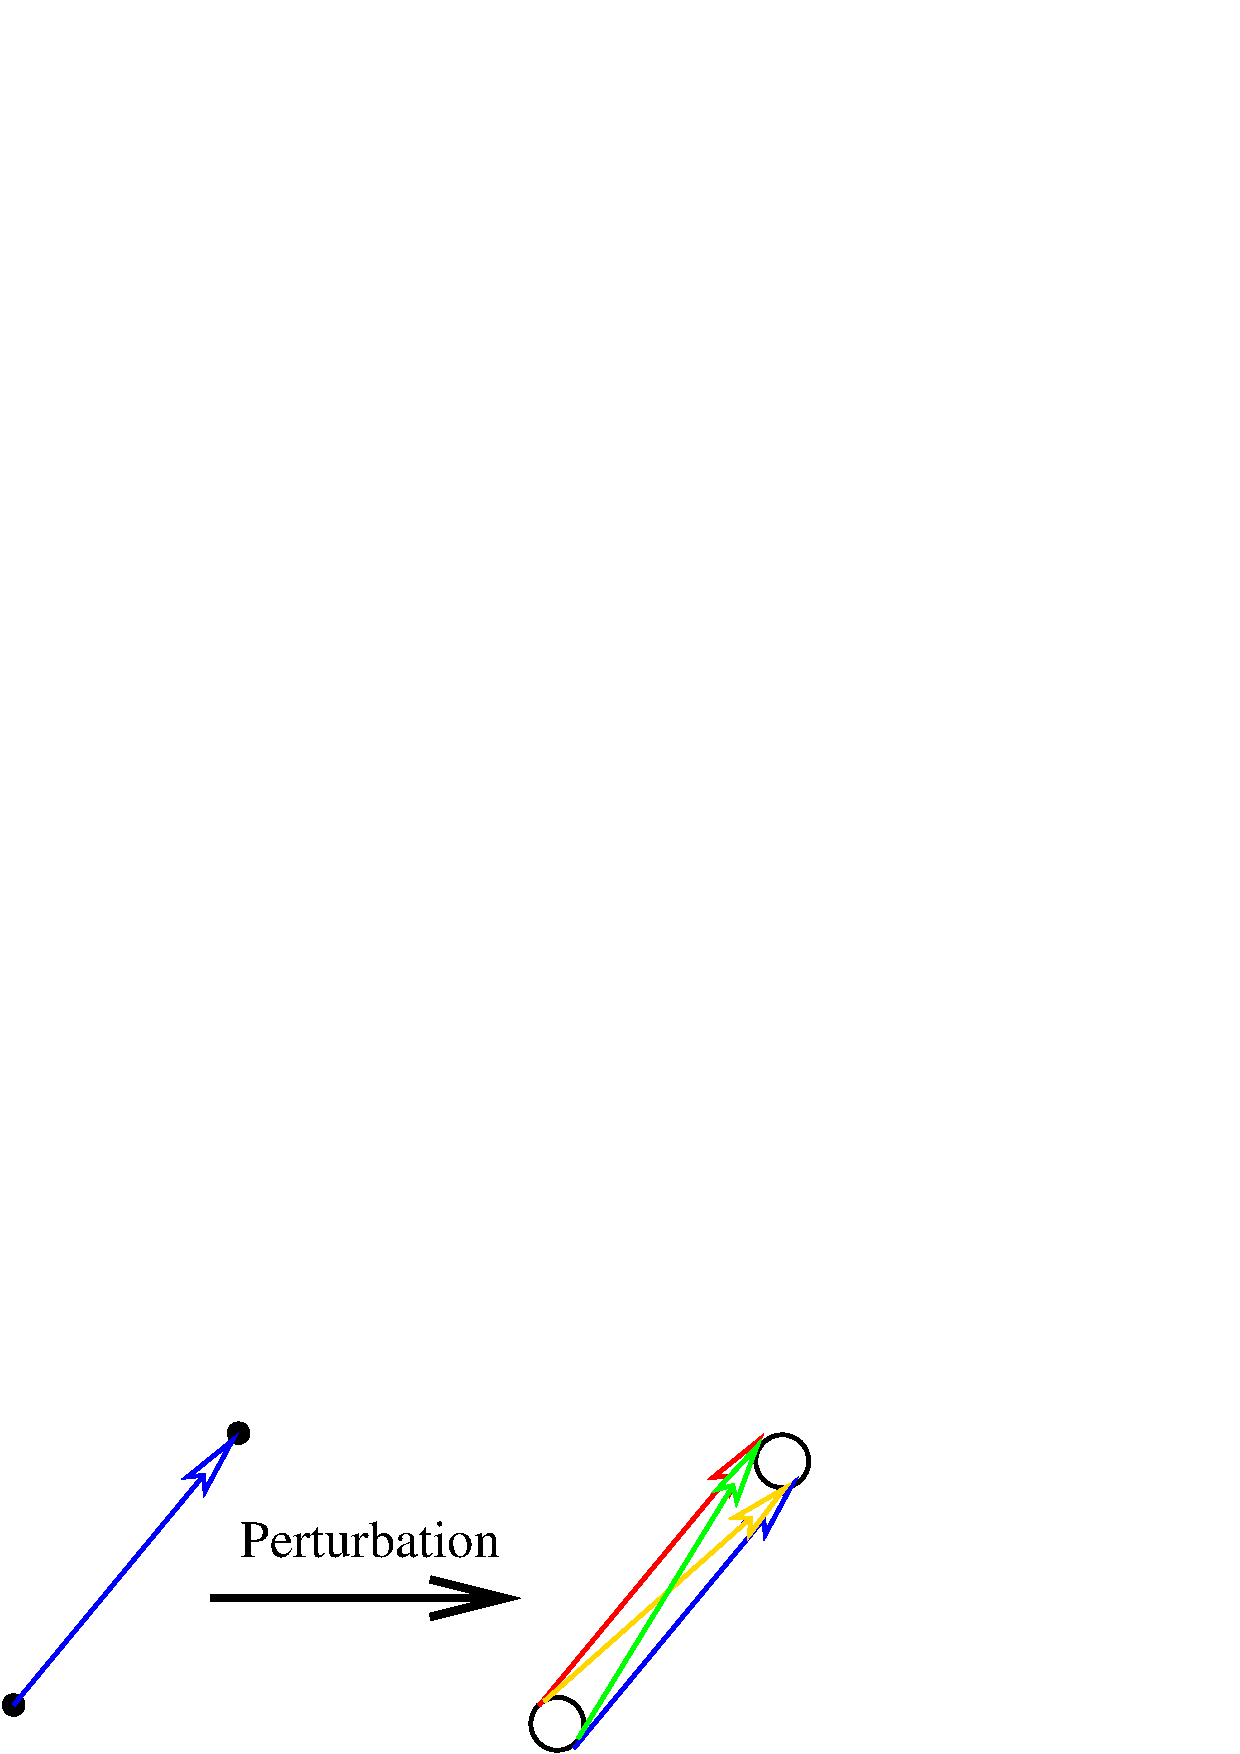
\includegraphics[height=4cm]{Visibility_complex_2/fig/points}%
    \end{center}
\end{ccTexOnly}

\begin{ccHtmlOnly}
    <CENTER>
        <img src="fig/points.gif" alt="Points"><P>
    </CENTER>
\end{ccHtmlOnly}

As an example, consider two points as in the figure above. They share four
bitangents which are geometrically equal. These four bitangent are
nevertheless represented by four different vertices in the visibility
graph. The order of the tangent points of these bitangents on the
"boundary" of the point is determined by the order of these tangent points
if the points were replaced by small circles. Considering the crossing
predicate, the \texttt{LR} and \texttt{RL} bitangents is the only crossing
pair in the figure above.  Also bear in mind that the presence of
degenerate cases may imply arcs with zero length.

\section{Using the package}

\subsection{Traits classes}
The classes in this package are templated by a geometric traits class that
specifies which kind of object is dealt with. Four traits classes are
provided:
\begin{itemize}
\item \ccc{Visibility_complex_2_point_traits<Kernel>}, defined in
file \ccc{CGAL/Visibility_complex_2/Point_traits.h}
\item \ccc{Visibility_complex_2_segment_traits<Kernel>}, defined in
file \ccc{CGAL/Visibility_complex_2/Segment_traits.h}
\item \ccc{Visibility_complex_2_polygon_traits<Kernel>}, defined in
file \ccc{CGAL/Visibility_complex_2/Polygon_traits.h}, for counterclockwise
oriented polygons
\item \ccc{Visibility_complex_2_circle_traits<Kernel>}, defined in file
\ccc{CGAL/Visibility_complex_2/Point_traits.h}, for circles with a
rational radius (a subclass of \ccc{Circle_2<Kernel>} (convertible to and from
\ccc{Circle_2<Kernel>}, generally with an approximation) is used).
\end{itemize}

A traits class defines a type \ccc{Disk} (the type of the convex objects
manipulated) and a class \ccc{Bitangent_2}. From an object of type
\ccc{Bitangent_2}, one can obtain its type (as defined in section
\ref{VC2-bit-type}) with the method \ccc{type()} and handles to its source
and target objects with the methods \ccc{source_object()} and
\ccc{target_object()}. The type of a bitangent is given as a value from the
nested enum type \ccc{Bitangent_2::Type}, containing values \ccc{LL},
\ccc{LR}, \ccc{RL}, and \ccc{RR}.

\subsection{Computing the free bitangents}
The class \ccc{Compute_free_bitangents_2<VC2GeomTraits>} implements a
function object that computes the set of free bitangents of a scene of
objects and possibly constraints. The main method, \ccc{operator ()} takes
as arguments a pair of iterators spanning the set of disks and an output
iterator through which the computed bitangents are returned.

This method only maintains a subset of the visibility complex with a size
linear in the size of the scene. If the output iterator (for instance, a
counting iterator) does not store (copies of) the bitangents, the total
memory used by the program will be linear, even if the visibility graph is
quadratic.

The following code sample computes the free bitangents of a set of segments
read from a file, and prints them on the standard output.

\ccIncludeExampleCode{Visibility_complex_2/segment_bit.cpp}

\subsection{Computing a visibility complex}

The class \ccc{Visibility_complex_2<VC2GeomTraits>} computes and stores a
visibility complex as defined in section \ref{VC2-vcdef}. The constructor
takes as argument a pair of iterators defining the sequence of disks, and
copies them into a container hidden in the constructed object (the
\ccc{source_object} and \ccc{target_object} handles in the computed
bitangents point into this container, not to the original objects).

The nested classes \ccc{Visibility_complex_2<VC2GeomTraits>::Edge},
\ccc{Visibility_complex_2<VC2GeomTraits>::Vertex}, and
\ccc{Visibility_complex_2<VC2GeomTraits>::Face} are used to represent the
edges, vertices and faces of the complex. The class \ccc{Vertex} is a
subclass of \ccc{VC2GeomTraits::Bitangent_2}, augmented with handles to
its incident edges and faces.

Iterators (\ccc{disks_begin}, \ccc{vertices_begin}, \ccc{edges_begin} and
\ccc{faces_begin} and their \ccc{*_end} counterparts) are provided to
browse through the complex. The methods \ccc{positive_edge} and
\ccc{negative_edge} can be used to find an unspecified edge supported by a
given object.

The following code sample computes the visibility complex of a set of
circles, and prints the bitangents incident to the first disk of the
sequence.

\ccIncludeExampleCode{Visibility_complex_2/vc_circle.cpp}



\section{General polygonal configurations}

Recall that disks, as they are defined above, are convex. We now describe
how to treat not only non convex polygons but also more general polygonal
configurations. Consider the general setting consisting in a family $S$ of
pairwise non crossing segments which are allowed to share an extremity. The
set $S$ can for example be the edges of a non-convex polygon.  We use the
following recipe to build a scene $T$ respecting our requirements:
\begin{itemize}
    \item Each extremity of a segment in $S$ is inserted as a point in $T$.
    Recall that points are treated symbolically as if they were small
    circles (see the paragraph above concerning degenerate cases).
    \item Each segment $s \in S$ directed from point $p$ to point $q$, with
    $p,q \in T$ is inserted in $T$ as a constraint directed from $p$ to
    $q$. The type chosen for the constraint (recall that four types are
    possible) is \texttt{RL}. The reason for this choice is to avoid two
    crossing constraints.
\end{itemize}

The Figure below shows a polygonal configuration $S$ and the scene $T$ which
has to be given as an input to our algorithms. 

\begin{ccTexOnly}
    \begin{center}
        \psfrag{S}{$S$}
        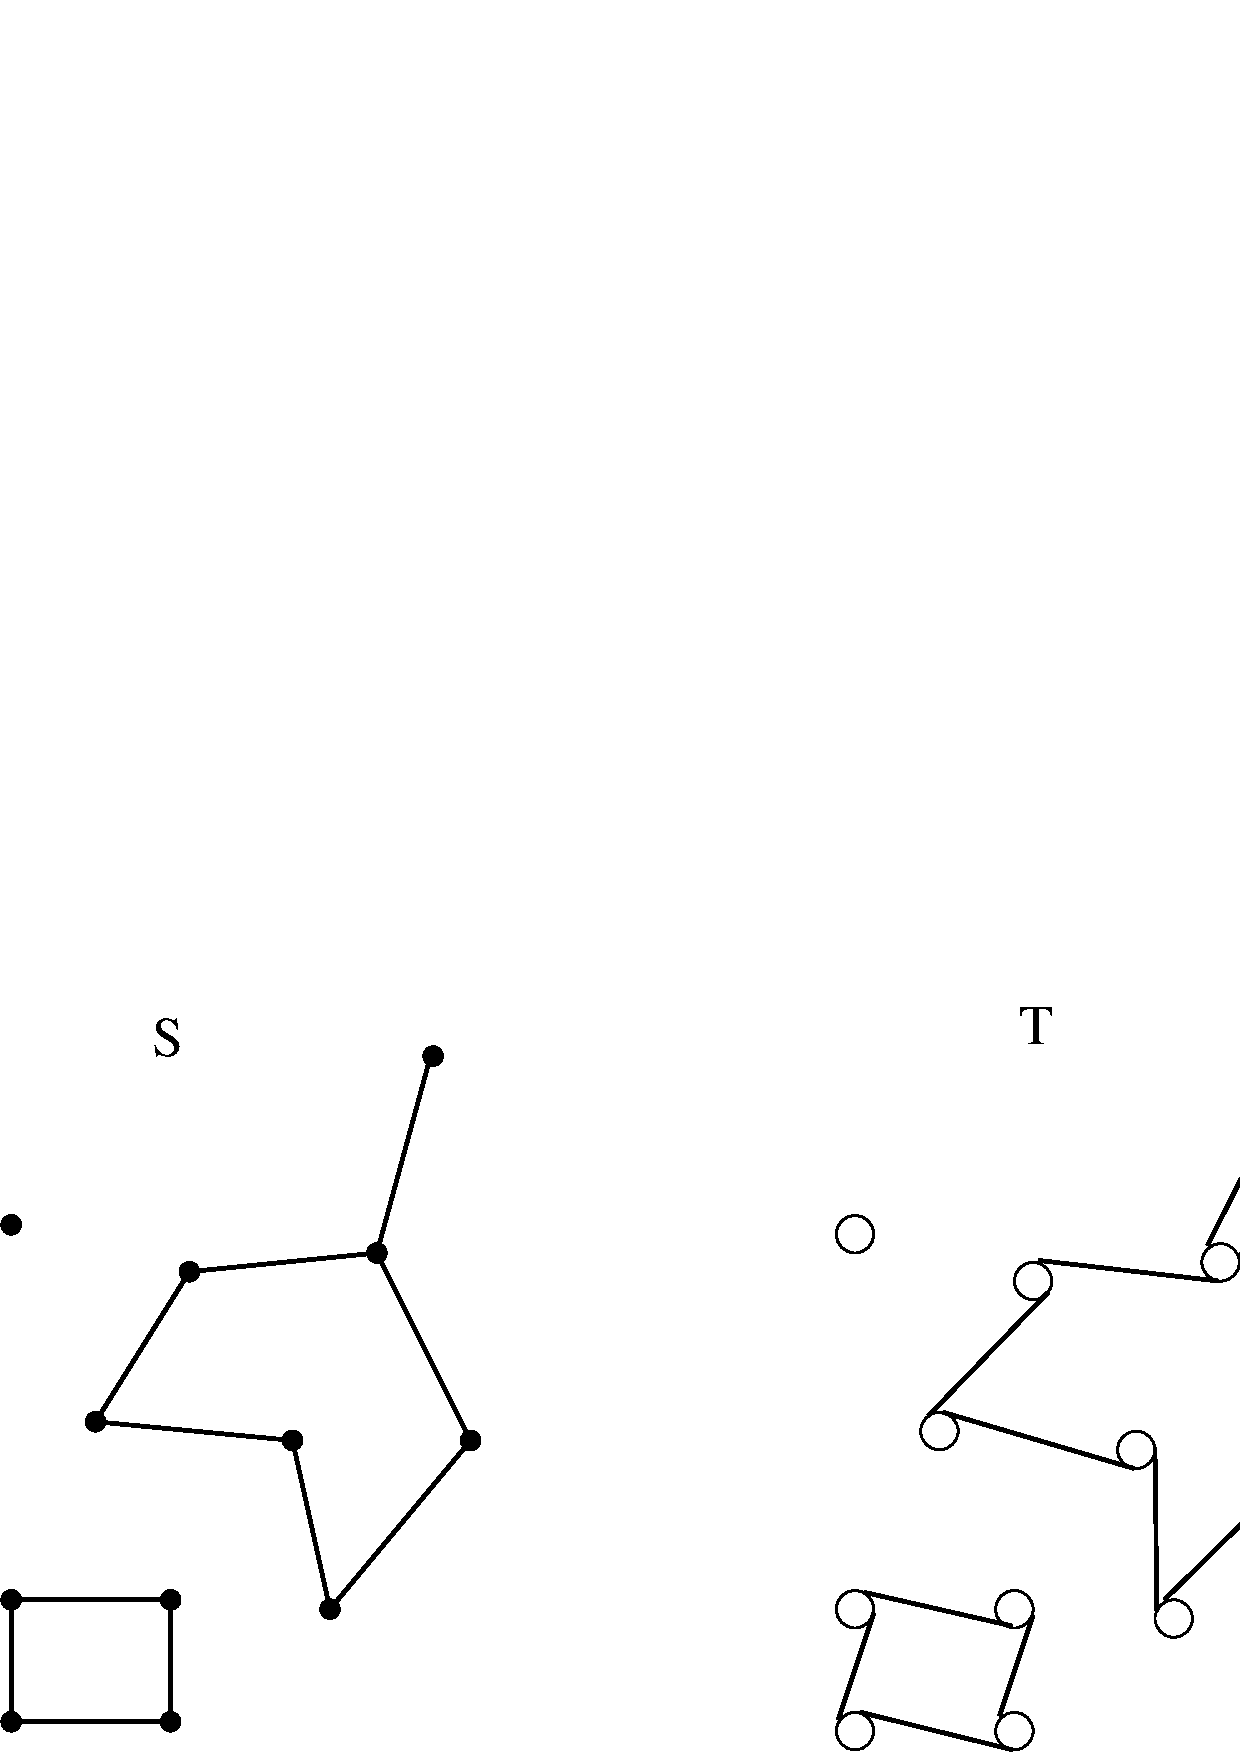
\includegraphics[height=8cm]{Visibility_complex_2/fig/configuration}%
    \end{center}
\end{ccTexOnly}

\begin{ccHtmlOnly}
    <CENTER>
        <img src="fig/configuration.gif" alt="Polygonal configurations"><P>
    </CENTER>
\end{ccHtmlOnly}

The constructor for \ccc{Visibility_complex_2<VC2GeomTraits>}, as well as
\ccc{Compute_free_bitangents_2<VC2GeomTraits>::operator()} can optionally
receive a third and fourth argument defining a sequence of
constraints, given as a value of a type accessible as
\ccc{Visibility_complex_2<VC2GeomTraits>::Constraint_input} or 
\ccc{Compute_free_bitangents_2<VC2GeomTraits>::Constraint_input}

The interface of the \ccc{Constraint_input} type is:
\begin{ccExampleCode}
class Constraint_input {
public:
  typedef Bitangent_2::Type Type;
  Constraint_input();
  Constraint_input(Type t,size_t source,size_t target);
  Type type() const;
  size_t source() const;
  size_t target() const;
};
\end{ccExampleCode}
It stores the type of the bitangent, and the index of the source and target
objects in the sequence of disks. An \ccc{operator >>} and an \ccc{operator
<<} are supplied.

For instance, this code reads a list of circles and a list of constraints
from files, and builds their visibility complex:
\ccIncludeExampleCode{Visibility_complex_2/constraints.cpp}

\section{Shortest paths}

The main goal of this package is to provide an implementation of the
visibility complex structure. However, since this is one of the main
applications of visibility graphs, we provide as an extra a class to
compute the shortest path between two points in a scene. 

This class, \ccc{Shortest_path_2<VC2GeomTraits>}, is defined in file
\ccc{CGAL/Shortest_path_2.h}. It is paramaterized by a geometric traits
class. \ccc{Visibility_complex_2_circle_traits} does not provide the
distance functions required for shortest path computations, and, therefore
cannot be used here, but the other traits classes (for points, segments and
polygons) can. By default, they use type \ccc{double} to compute the
distances. It is possible to have them use an exact type by passing this
type as the second template paramater of the traits class, along with a
conversion functor as third, but very poor performance is to be expected,
since large sums of square roots are going to be compared.

\ccc{Shortest_path_2<VC2GeomTraits>} exports a nested class
\ccc{Visibility_complex_2}, which is a specialisation of
\ccc{Visibility_complex_2<VC2GeomTraits>} (with extra fields in the edges
and vertices). The constructor for \ccc{Shortest_path_2<VC2GeomTraits>}
takes as argument an object from this class \ccc{Visibility_complex_2},
which should be built over the set of obstacles, and the set of points
between which shortest paths are to be computed (converted into
\ccc{VC2GeomTraits::Disk} using functor
\ccc{VC2GeomTraits::Make_convex_from_point}). Once the object is
initialised, its method \ccc{void compute_shortest_paths(const Disk& s)}
should be called to compute the shortest path starting from its argument
(which is assumed to be a point converted to a
\ccc{VC2GeomTraits::Disk}). Then, for each target point, the methods
\ccc{get_path_vertices} and \ccc{get_path_bitangents} can be used to
retrieve the shortest path to this point. They take as first argument the
target point, and, as second argument, an output iterator through which the
list of bitangents is returned. In the case of \ccc{get_path_vertices}, the
output iterator receives handles to vertices of the complex, while with
\ccc{get_path_bitangents}, the output iterator receives copies of the
underlying bitangents (type \ccc{VC2GeomTraits::Bitangent_2}).

For instance, the following code computes a shortest path between two
points in a scene made of three segments.

\ccIncludeExampleCode{Visibility_complex_2/shortest_path.cpp}

\section{Augmenting the edges, vertices and faces}

It is possible to customize the edges, vertices and faces. The classes
\ccc{Visibility_complex_2} and \ccc{Shortest_path_2} accept an extra
template argument, which should be a model of concept \ccc{VC2Items}. It
provides bases for edges, vertices, and faces. Here is the skeleton of an
items class~:

\begin{ccExampleCode}
class Items {
  template <class A> class Vertex_wrapper {
    class Vertex {
      // A model of concept VC2Vertex
    };
  };
  template <class A> class Edge_wrapper {
    class Edge {
      // A model of concept VC2Edge
    };
  };
  template <class A> class Face_wrapper {
    class Face {
      // A model of concept VC2Face
    };
  };
}
\end{ccExampleCode}

The template argument \ccc{A} is instantiated with a class exporting the
final types \ccc{Edge}, \ccc{Vertex} and \ccc{Face} used in the complex
(which are derived from the classes \ccc{Edge}, \ccc{Vertex} and \ccc{Face}
defined here).

Two items classes are provided~: \ccc{Visibility_complex_2_items} and
\ccc{Shortest_path_2_items}. The former is the most basic one, while the
latter provides edges and vertices with extra fields to help compute the
shortest paths.

To define your own items class, you should derive from one of the default
items classes, and inside it, define \ccc{Edge}, \ccc{Vertex} and
\ccc{Face} classes derived from those defined in the base itemps class.
